\chapter{Related Work}
This chapter gives an overview of the bazo cryptocurrency and its underlying blockchain technology. Additionally it presents an analysis of blockchain explorers for 2 different cryptocurrencies, highlighting both similarities and differences in the implementation and functionality of the applications. The analysis plays a major role in the specification of the Bazo Blockchain Explorer, as it helps making design decisions for requirements.

\section{The Bazo Blockchain and Cryptocurrency}
Developed in 2017 at the University of Zurich, the Bazo cryptocurrency is a private blockchain that aims to reduce administrative overhead, as well as extend the functionality of a financial service provider's bonus point reward system. Traditionally, for each merchant who wants to sell its products in the rewards shop of the service provider, specific contracts between the two parties need to be made. This makes expanding the bonus point system a time and resource consuming process. Bazo eliminates this restriction by introducing a cryptocurrency which allows to directly make transactions between merchants and users or even between users itself using Bazo Coins. The merchants itself do not need to form contracts with the service provider anymore, they can offer their products in exchange for Bazo Coins even at their own PoS. The only interaction between the service provider and merchants consist of the exchange of Bazo Coins for fiat currency. Users of the bonus point system can exchange their current bonus points for Bazo coins. In order to access the blockchain, client and miner applications are available. Simultaneous to the development of the Bazo Blockchain Explorer, a light client and a payment app were developed as well.

\section{Existing Blockchain Explorers and Analytics Platforms}
\subsection{Blockexplorer.com}
This blockchain explorer was built for both the bitcoin and bitcoin cash blockchain. The frontend of the web application is called Insight UI and is built using AngularJS, a javascript framework. It interacts with the Insight API, the corresponding backend. Insight API consists of a REST and websocket API for Bitcore Node, a query and indexing service for the bitcoin blockchain. The source code for both frontend and backend are available on GitHub.

\begin{figure}
  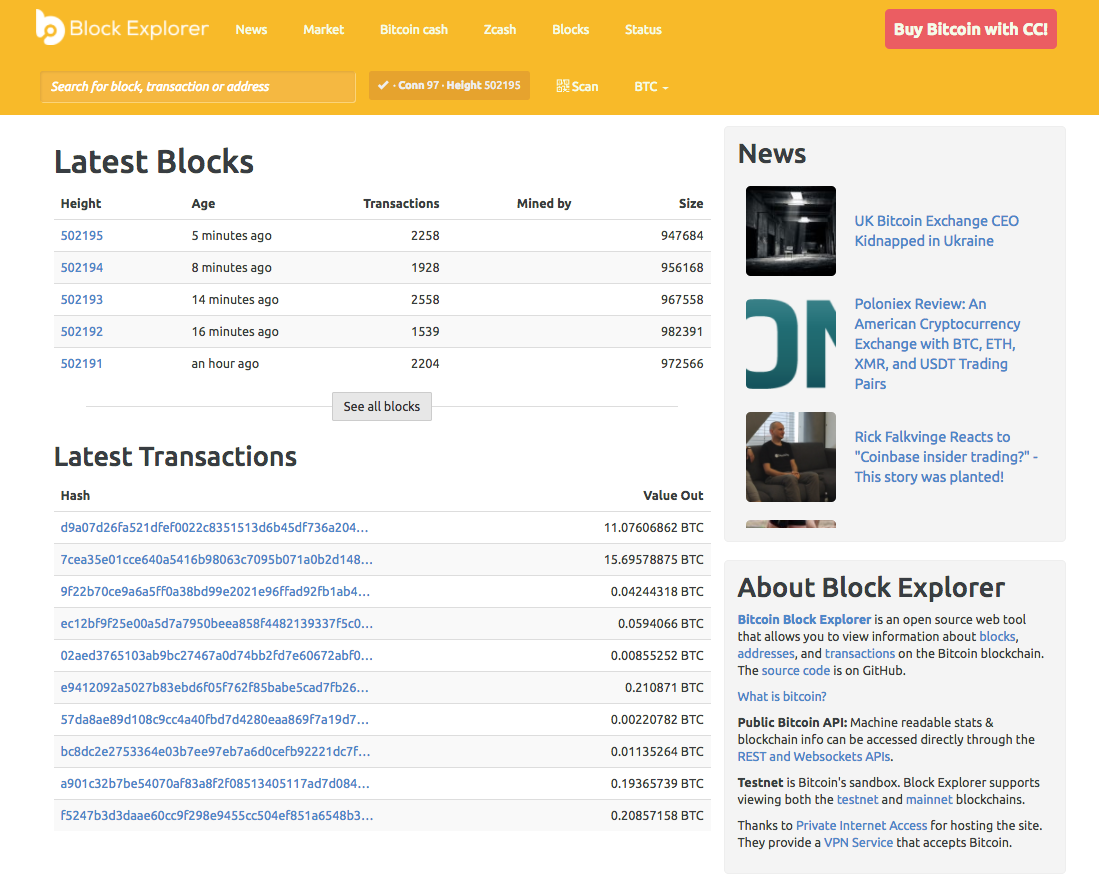
\includegraphics[width=\linewidth]{blockexplorer.png}
  \caption{Landing page of blockexplorer.com}
  \label{fig:blockexplorer1}
\end{figure}

\subsection{Etherscan.io}
EtherScan is a block explorer and statistics analysis platform for the ethereum blockchain. It uses Go Ethereum, an implementation of the Ethereum protocol in the Go language, in combination with Parity, a client for interacting with the Ethereum blockchain. EtherScan is a closed source project.

\begin{figure}
  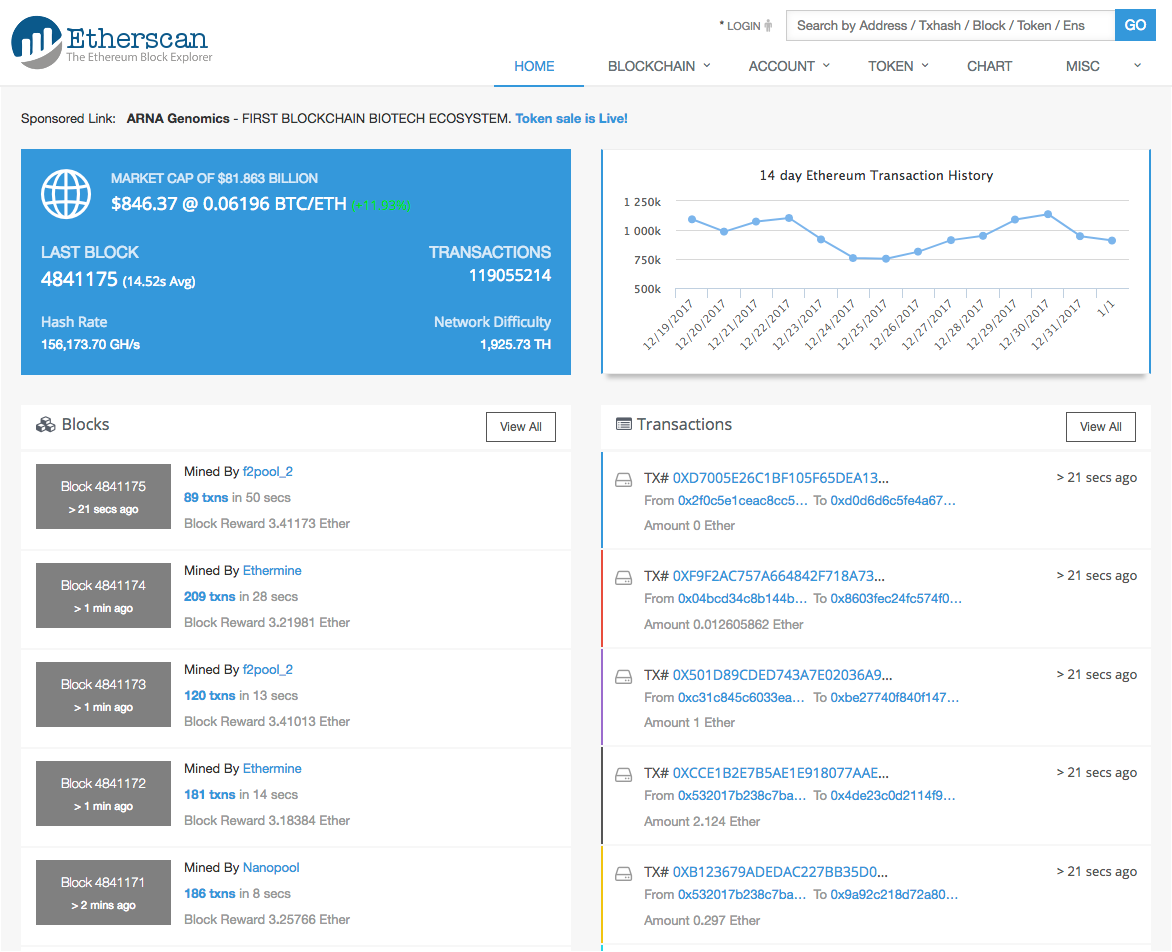
\includegraphics[width=\linewidth]{etherscan.png}
  \caption{Landing page of etherscan.io}
  \label{fig:etherscan1}
\end{figure}

\section{Analysis}
This analysis omits features of the explorers that do not relate to the blockchain itself, such as newsfeeds of blockchain-related topics or social media links. Both explorers offer similar functionality as their core-feature: Structured views of blocks and transactions. The landing pages display the most recently mined blocks and transactions, with blockexplorer offering real-time updates. EtherScan also displays statistical data about the chain, such as the market cap, mining difficulty and hash rate. A search feature is present on both sites, offering the user to search for transactions, blocks and accounts via their respective hashes. To browse the chain, links are used extensively (e.g. every block on the landing page links to its respective detailed block page). When presenting multiple objects on the same page, such as a list of blocks, the data is structured using tables, in EtherScan's case using pages with a predefined length and in blockexplorer's case using a date picker that displays all blocks which have been mined on the chosen date. When multiple items are displayed using lists, less information about the items is given, compared to when a single item is viewed.

\subsection{Requirements for the Bazo Blockchain Explorer}
\subsubsection{Navbar}
A navbar lets the user jump to all functionality of the website. The 